%% Template for MLP Coursework 1 / 16 October 2017 

%% Based on  LaTeX template for ICML 2017 - example_paper.tex at 
%%  https://2017.icml.cc/Conferences/2017/StyleAuthorInstructions

\documentclass{article}

\usepackage[T1]{fontenc}
\usepackage{amssymb,amsmath}
\usepackage{txfonts}
\usepackage{microtype}
\usepackage{enumitem}

% For figures
\usepackage{graphicx}
\usepackage{subfigure} 

% For citations
\usepackage{natbib}

% For algorithms
\usepackage{algorithm}
\usepackage{algorithmic}

% the hyperref package is used to produce hyperlinks in the
% resulting PDF.  If this breaks your system, please commend out the
% following usepackage line and replace \usepackage{mlp2017} with
% \usepackage[nohyperref]{mlp2017} below.
\usepackage{hyperref}
\usepackage{url}
\urlstyle{same}

% Packages hyperref and algorithmic misbehave sometimes.  We can fix
% this with the following command.
\newcommand{\theHalgorithm}{\arabic{algorithm}}


% Set up MLP coursework style (based on ICML style)
\usepackage{mlp2017}
\mlptitlerunning{MLP Coursework 1 (\studentNumber)}
\bibliographystyle{icml2017}


\DeclareMathOperator{\softmax}{softmax}
\DeclareMathOperator{\sigmoid}{sigmoid}
\DeclareMathOperator{\sgn}{sgn}
\DeclareMathOperator{\relu}{relu}
\DeclareMathOperator{\lrelu}{lrelu}
\DeclareMathOperator{\elu}{elu}
\DeclareMathOperator{\selu}{selu}
\DeclareMathOperator{\maxout}{maxout}

%% You probably do not need to change anything above this comment

%% REPLACE this with your student number
\def\studentNumber{s1, s2, s3}

\begin{document} 

\twocolumn[
\mlptitle{MLP Coursework 3: Project Interim Report}

\centerline{\studentNumber}

\vskip 7mm
]

\begin{abstract} 
The abstract should be 100--200 words long,  providing a concise summary of the contents of your report. \textbf{still needs to be written.}
\end{abstract} 

\section{Introduction and Motivation}
\label{sec:intro}

During the last years, connectionist based approaches have gained popularity to solve computer vision tasks \cite{dinsmore2014symbolic}. A significant number of convolutional neural networks architectures have emerged since they demonstrated their power in the 2012 ImageNet Large-Scale Visual Recognition Challenge (ILSVRC) \cite{krizhevsky2012imagenet}. Several factors have contributed to extend the development of this kind of solutions including an increase in the amount of available training data \cite{simonyan2014very}, more compute power \cite{Szegedy_2015_CVPR}, and better software abstraction layers.

Although deep neural networks work well with large amounts of training data \cite{lotsDataAndrew}, the performance of these models typically decreases in situations where only small amounts of training data is available [INSERT REFERENCE TO LEARNING CURVE HERE]. This poses a problem to solve computer vision tasks where the amount of data is not appropiate to utilise these emergent technologies. In addtion, the amount of information extracted from images (features) also impacts the performance of a model. This situation means that a given system would not be suitable to solve the same task with other data.

There exists a number of data manipulation methods that try to reduce the impact of small datasets. Some alternatives simply perform data augmentation \cite{krizhevsky2012imagenet}, whereas others implement more advanced techniques like data synthesize \cite{hu2018frankenstein}. Recently, some approaches have tried to address this problem using novel techniques within the domain of deep neural networks including transfer learning \citep{ng2015deep}, \cite{oquab2014learning}. and deep features extraction \citep{chen2016deep}.

In this report, we aim to explore how the size of datasets and the information from images impact in the performance of a given convolutional neural network. The work described here will be the foundation for further investigations of machine learning techniques e.g., transfer learning and deep features extraction \footnote{These techniques have other use cases that are not necessarily explored within this paper.}, to boost the performance of deep neural network architectures under conditions of small data.

We present and analyse the results of reducing the training set size using two different and comparable datasets. The methodology includes performing an observation of the accuracy of the proposed architecture as the training size is decreased (\ref{sec:methodology}); this procedure is applied to both datasets. The datasets were selected based on the visual perception of differences between classes; in the first one the differences are easily perceived, whereas in the second one, classes have subtle differences.

Within the remainder of this paper, we present a set of research questions and associated hypotheses (\ref{sec:questions}). Later, an overview of the selected datasets and the task is documented (\ref{sec:data}). Subsequently, the methodology employed to address the aforementioned research questions and hypotheses are outlined (\ref{sec:methodology}) and experimental results are documented (\ref{sec:baseline}) which are then draw upon to derive a set of initial conclusions (\ref{sec:conclusions}). Finally, details of any associated risks, backup plans and further work are provided (\ref{sec:future}).

 
\begin{table*}[!htb]
  \centering
  \begin{tabular}{| l | l | l | l | l | l | l |}
    \hline
    \textbf{Dataset} & \textbf{Number of classes} & \textbf{Training size} & \textbf{Test size}  &  \textbf{Sample per class} & \textbf{Samples size} & \textbf{Format} \\ \hline
    Clothes & 7 & 42000 & 7000 & 7000 & 64x64 & Grayscale\\ \hline
    Faces & 7 & 42000 & 6300 & 6900 & 64x64 & Grayscale\\ \hline
  \end{tabular}
  \caption{Characteristics of datasets}
  \label{tab:1}
\end{table*}

\section{Research Questions}
\label{sec:questions}

As described in (\ref{sec:arch}), there are two aspects of data that can impact the performance of neural networks: size and features. These variables are the base for the research questions that we explore later on. 

Here, we present research questions addressed within this report (\ref{sec:irquestions}), future research questions for the next stage of the project(\ref{sec:frquestions}), and hypotheses(\ref{sec:hypotheses}).

\subsection{Interim Research Questions}
\label{sec:irquestions}

\begin{enumerate}
  \item How do visually perceived differences among classes affect the accuracy of the proposed convolutional neural network architecture (\ref{sec:arch})?
  \item How does reducing the size of a training dataset affect the performance of the proposed convolutional neural network architecture?
\end{enumerate}

In regards to the first question, humans can easily identify different objects based on their visual characteristics. This situation is true for elements which attributes are quite different from one to another (pieces of clothing) as well as for those which differences are subtle (facial expressions). 

We are interested in explore how the visually perceived similarity of different classes can affect the performance of a neural network. Although we do not provide a similarity metric among instances of data, we comment about this topic as a potential future work (\ref{sec:future}).

It is commonly thought that small datasets lead to poor generalisation \cite{lotsDataAndrew}. The second research question links into our future research questions (\ref{sec:frquestions}) associated with using machine learning techniques to improve the performance of neural network architectures under small data conditions.

\subsection{Future Research Questions}
\label{sec:frquestions}

\begin{enumerate}
  \item How does the application of transfer learning affect the performance of the proposed neural network architecture under different sizes of the datasets?
  \item How does the application of deep features extraction affect the performance of the proposed neural network architecture under different sizes of the datasets?
\end{enumerate}

\subsection{Hypotheses}
\label{sec:hypotheses}
\begin{enumerate}[label=\textbf{H.\arabic*}]
  \item \label{h:1} The proposed convolutional neural neural network (\ref{sec:arch}) has a better performance when the visually perceived differences among classes are high.
  \item \label{h:2} The proposed convolutional neural neural network (\ref{sec:arch}) reduces its performance when the size of the training set is reduced. 
 \end{enumerate}

\section{Datasets and Task}
\label{sec:data}

We selected two datasets based in the visually perceived differences among their classes: 
\begin{itemize}
  \item Fashion-MNIST \citep{DBLP:journals/corr/abs-1708-07747}
  \item Facial Expression Research Group Database (FERG-DB)\citep{aneja2016modeling}
\end{itemize}

Fashion-MNIST (hereafter referred as clothes dataset) as stated by their authors "it is intended to serve as a direct drop-in replacement for the original MNIST dataset for benchmarking machine learning algorithms." This situation means that the dataset shares the same characteristics with its predecessor. It contains 70000 grayscale images of size 28x28 distributed among 10 classes. The training and test sets have 60000 and 10000 samples, respectively.

FERG-DB (hereafter referred as expressions dataset) contains 55767 colorful labeled images of size 256x256. The images depict six individually stylized characters with one of out seven facial expressions: anger, disgust, fear, joy, neutral, sadness and surprise.

As mentioned, the visually perceived differences among the classes in the datasets are different. In the cases of the clothes dataset, it is clearly evident that the main difference between the samples of different classes is the contour as seen in Figure (\ref{fig:1}). Unlike clothes, facial expressions requires subtle changes in the geometry of a face. The overall structure of a face is similar in every expression, however, the shapes of its components (mouth, eyes, eyebrows, etc) change as seen in Figure (\ref{fig:2}).
\begin{figure*}[tb]
	\vskip 5mm
		\begin{center}
			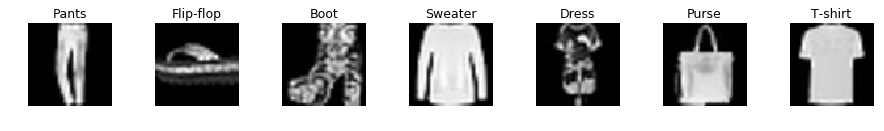
\includegraphics[width=\textwidth,height=2.5cm]{original_clothes}
			\caption{Samples of classes in clothes dataset. For easy understanding, we have labeled the classes with words}
			\label{fig:1}
		\end{center}
	\vskip -5mm
\end{figure*}

\begin{figure*}[tb]
	\vskip 5mm
		\begin{center}
			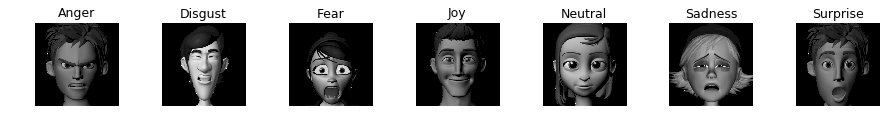
\includegraphics[width=\textwidth,height=2.5cm]{original_expressions}
			\caption{Samples of classes in expressions dataset. Each of the six characters is displayed}
			\label{fig:2}
		\end{center}
	\vskip -5mm
\end{figure*}

\subsection{Preprocessing}
\label{sec:preprocessing}
We preprocessed both datasets to be able to have similar characteristics as seen in Table (\ref{tab:1}). Since the expressions dataset contains seven classes, we reduced the number of classes of the clothes dataset to the same value. Later we split the expressions dataset into training and test sets. After this process, the clothes dataset ended up with 42000 and 7000 samples for the training and test sets evenly distributed among the seven classes. 

A similar situation occured for the expressions dataset with 42000 and 6300 samples for the training and test sets respectively. In addition, the images in this dataset were converted from colorful to grayscale. Finally, all the images from both datasets were resized to 64x64, this size allows to maintain the relevant features for the facial expressions without increasing too much the computational resources in the training stage.

Finally, a series of transformations was performed in the test sets samples in order to increase the variability of the images. Rotation, blur, skew and shift transformations were randomly applied to each image as seen in Figures (\ref{fig:3}) and (\ref{fig:4}).

\begin{figure*}[!htb]
	\vskip 5mm
		\begin{center}
			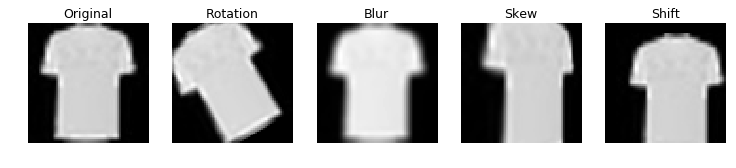
\includegraphics[height=2.5cm]{augmented_clothes}
			\caption{Transformations applied to samples in clothes test set}
			\label{fig:3}
		\end{center}
	\vskip -5mm
\end{figure*}

\begin{figure*}[!htb]
	\vskip 5mm
		\begin{center}
			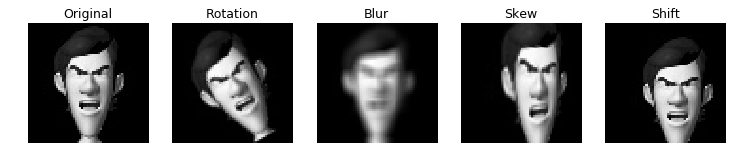
\includegraphics[height=2.5cm]{augmented_expressions}
			\caption{Transformations applied to samples in expressions test set}
			\label{fig:4}
		\end{center}
	\vskip -5mm
\end{figure*}

\subsection{Task and Evaluation}
\label{sec:evaluation}
We set a classification task based on the labels provided by the datasets. Each experiment is evaluated based on the validation accuracy obtained in the last iteration of the training process. We compare the results of the experiments in two ways: comparison of the accuracy through different sizes of each dataset, and comparison of the accuracy between the same sizes of both datasets.

\section{Methodology}
\label{sec:methodology}
We examine the interim research questions (\ref{sec:irquestions}) to create a neural network architecture (\ref{sec:arch}). Based on our hypotheses, there are two main variables that we handle in every experiment: the dataset and its size. This means that the rest of elements in the system like the hyper-parameters, activation functions, optimization strategies and else are kept constant.

There are two kind of experiments to perform. In the first one we select one dataset to train the model. The other type of experiments correspond to the size of the selected dataset. When performing the second kind of experiments, we use the same samples for the validation stage to make proper comparisons of the accuracy. To do so, we utilise the test sets that we preprocessed earlier.


\subsection{Proposed Neural Network Architecture}
\label{sec:arch}

We use a simple architecture containing one convolutional which is flattened and connected to a dense layer. The objective of this shallow structure is to have a model that extracts features at the same level in different datasets. We have to remember that the visually perceived differences in the clothes dataset are higher than in the expressions dataset. Based on this, a deeper architecture might be able to extract more features from both datasets but that information would be more relevant for the expressions than for clothes.

Finally, relu and softmax activations along with max pooling layers are integrated into the structure of the network. The weights and biases of the convolutional layer are initialised with uniform distributions, whereas the parameters of the dense layer are initialised using the glorot strategy. The Adam learning rule is used to reduce the error of the system.  The total number of training parameters of the network is 31637. 


\section{Baseline Experiments}
\label{sec:baseline}

\begin{table*}[!htb]
  \centering
  \begin{tabular}{| l | l | l |}
    \hline
    \textbf{Size} & \textbf{Accuracy for clothes} & \textbf{Accuracy for expressions}\\ \hline
    100\% & 0.51 & 0.34\\ \hline
    75\% & 0.53  & 0.34\\ \hline
    50\% & 0.51 & 0.35\\ \hline
	25\% & 0.52 & 0.34\\ \hline
	10\% & 0.55 & 0.34\\ \hline
	1\% & 0.50 & 0.32\\ \hline

  \end{tabular}
  \caption{Validation accuracies for different sizes of the datasets}
  \label{tab:2}
\end{table*}

\begin{table*}[!htb]
  \centering
  \begin{tabular}{| l | l | l |}
    \hline
    \textbf{Size} & \textbf{Accuracy for clothes} & \textbf{Accuracy for expressions}\\ \hline
    100\% & 0.76 & 0.49\\ \hline
    75\% & 0.78  & 0.49\\ \hline
    50\% & 0.76 & 0.48\\ \hline
	25\% & 0.74 & 0.47\\ \hline
	10\% & 0.78 & 0.50\\ \hline
	1\% & 0.76 & 0.44\\ \hline

  \end{tabular}
  \caption{Validation accuracies for different sizes of the datasets using data augmentation}
  \label{tab:3}
\end{table*}


\section{Interim Conclusions}
\label{sec:conclusions}

TODO

\section{Future Work}
\label{sec:future}
Draft by Steven:
In the second phrase of the project, two different transfer learning methods will be studied to examine potential methods to improve performances given very small dataset which is frequent in real-world scenario. Firstly, we transfer a very large pre-trained network VGG16 on our aforementioned baseline system with pre-trained weights on small dataset. Since VGG16 trains on 200 types of general objects. The generality of the model might be beneficial to train on common objects (clothes dataset). Apart from transferring model to domain-specific dataset (clothes dataset). We also transfer the model to dataset with unrelated and subtle differences between classes in the dataset (facial dataset), to test the effectiveness of pre-trained model on task that shares little similarity with the pre-trained model.

Besides transferring pre-trained model, we also wish to investigate the effect of one-shot learning on small dataset. To demonstrate a basic version of one-shot learning we will implement Siamese network on either one of the dataset( clothes/facial expression) with the help of existing models and our modification to these models , due to time constrain and taking potential difficulty of implementing one-shot learning architecture from scratch. As a backup plan, we will abandon this experiment and focus more on transferring models methods.


\subsection{Backup Plans}
\label{sec:plans}

TODO


\bibliographystyle{abbrv}
\bibliography{biblo.bib}

\end{document}